\documentclass[10pt,letterpaper]{article}
\usepackage[margin=0.72in]{geometry}
\usepackage{booktabs,graphicx,hyperref,array}
\hypersetup{colorlinks=true,urlcolor=blue,linkcolor=black,
 pdftitle={Cloud Management for Energy and Performance},
 pdfsubject={Four-policy scheduler implementation and measured comparative study}}
\emergencystretch=2em
\setlength{\parindent}{0pt}
\setlength{\parskip}{5pt}
\setlength{\tabcolsep}{5pt}
\newcommand{\policies}{RR (round robin), BF (best fit), MP (minimum power), and DE (deadline energy)}
\begin{document}
\begin{center}
{\Large Cloud Management for Energy and Performance}\\[4pt]
{\large Four scheduling policies in the supplied cloud simulator}\\[3pt]
Comparative implementation report \quad November 8, 2026
\end{center}

\section*{Implementation and algorithms}
The objective is to reduce cluster energy while meeting each task class's SLA.
The delivered implementation changes \texttt{Scheduler.cpp}, retains every supplied
header and simulator object. The environment variable
\texttt{SCHEDULER\_POLICY} selects the algorithm. Initialization discovers the machine count, CPU families,
cores, memory, accelerators, and power/performance tables. It makes no assumptions
about machine numbering, a fixed cluster size, or Linux/x86-only work.

\textbf{RR: capacity-aware round robin.} Tasks go to the next compatible host
with a free core and sufficient memory. All machines remain in S0 and execute at
P0. This is a reproducible baseline with the same admission safeguards as the
energy policies, rather than the supplied skeleton's hard-coded placement and
unconditional migration.

\textbf{BF: best-fit consolidation.} Prefer an already occupied host with the
largest fraction of occupied cores. Otherwise choose an empty host in identifier
order. Tasks execute at P0; idle hosts enter S1, retaining one S0 standby per CPU
family. Consolidation reduces the number of machines that must leave sleep.

\textbf{MP: online incremental-power placement.} This policy adapts the placement
rule in Beloglazov, Abawajy, and Buyya's Modified Best Fit Decreasing (MBFD)
algorithm~[1]: choose a feasible host with the least added power. Here an arriving
task is the placement unit. Its estimated increase includes busy-core power minus
idle-core power, and, for an empty non-standby host, the machine and core power
increase from S1 to S0. It uses P0 and the same idle policy as BF. This is an
\emph{online adaptation}: it omits MBFD's batch sorting of VMs and the paper's
migration policies. No claim is made to reproduce the paper's experimental results.

\textbf{DE: deadline-aware execution-energy placement and DVFS (default).} For
each candidate host, evaluate every P-state and protect every assigned task with
an SLA. With remaining instructions $I_i$ and host speed $f_p$ in MIPS, service
is estimated as $r_{i,p}=I_i/f_p$ microseconds. A state is feasible when
$1.1r_{i,p}+120{,}000+w\le d_i-t$ for each guaranteed task, where $w=0$ on a ready
host and $420{,}000$ microseconds otherwise. The state minimizes
\[
 E_p=\big[(P_{S0}+C P_{C1})\max_i r_{i,p}
             +(P_p-P_{C1})\sum_i r_{i,p}\big]/10^6.
\]
This includes static energy while work executes. Placement minimizes the increase
in this estimate; GPU-capable work receives a 0.1 score multiplier on GPU hosts.
GPU speedup is deliberately omitted from deadline bounds, making them conservative.
If no candidate meets the bound, P0 and minimum predicted service plus wake delay
provide a progress fallback. Frequency is reconsidered on admissions, completions,
and periodic checks; all cores change together, as required by the interface.

\textbf{Shared safeguards.} CPU and VM types must match. Each distinct VM image
uses 8 MB overhead, counted along with task memory \emph{before} reserving a host
that is waking. Admission permits at most one task per core. Excess requests wait
in earliest-deadline order; best-effort jobs gain admission rank and task priority
after twice their nominal service time. State-completion callbacks gate VM
attachment. Empty VMs are reclaimed after completion bookkeeping. Hosts with work
are never put to sleep. These policies avoid migration and its latency entirely.
Requests impossible on every machine fail explicitly; admitted tasks are never dropped.

\newpage
\section*{Experimental design}
The simulator supplies random task generation, the event queue, VM execution, CPU
scheduling, and energy metering. Reimplementing these supplied components would
change the experiment. The scheduler uses only the public interfaces; knowledge
of future task arrivals is not used in placement or power decisions.

Five new workloads were generated by \texttt{tools/generate\_workloads.py}; their
complete, directly runnable inputs are in \texttt{input\_files/custom/}.
\begin{center}
\small
\begin{tabular}{p{1.17in}p{1.38in}p{3.75in}}
\toprule
Input & Cluster & Question tested \\
\midrule
02\_low\_intensity & 8 x86, 4 cores each & Sparse 0.3 s requests; can unused hosts sleep? \\
03\_surge & 12 x86, 4 cores each & Two bursts at 3--5 s and 8--10 s; 12 ms average arrivals, 2 s SLA0 jobs. \\
04\_heterogeneous & 12 hosts; x86, ARM, POWER, RISC-V & All four VM images; GPU/non-GPU x86 hosts, mixed SLA classes, and architecture constraints. Suggested input-file submission. \\
05\_memory\_pressure & 3 x86, 4 cores, 96 MB each & Two VM types and 48 MB nominal task memory; memory limits admission before cores do. \\
06\_dvfs\_slack & 4 x86, 8 cores each & SLA2 work with 80/24/10/4 W core P-states; when does slowing cores save energy? \\
\bottomrule
\end{tabular}
\end{center}

The main study runs these five scenarios plus the supplied NiceAndSmooth-1 and
SpikeyNefarious-1, with all four policies. Every original task-class seed is used
with offsets 0, 101, and 202, giving $7\times3\times4=84$ independent simulator
executions. Each policy sees the same generated workload within an input/seed pair.
The seed offsets are applied to every task class, preserving the workload's
configuration. Three runs expose seed sensitivity but do not establish statistical
generalization. Low-intensity samples contain only 8--20 tasks per seed.

\textbf{Metrics and reproducibility.} Energy comes from
\texttt{Machine\_GetClusterEnergy()} in kWh. Simulated makespan is the final
simulation timestamp in seconds; wall time is separately measured using Python's
monotonic performance counter. Mean response includes admission and wake delays.
The raw CSV also records mean response divided by the task's exposed
\texttt{target\_completion-arrival}, excluding best-effort SLA3, and per-SLA
populations. A zero miss percentage for an absent SLA class is not evidence of
compliance. The allowed miss rates for populated SLA0/1/2 classes are 5/10/20\%.

Every execution retains its precise \texttt{RESULT} record and input SHA-256.
\texttt{make benchmark} reproduces the main study. The README gives commands for
the additional supplied workloads. Tables are generated from the saved CSV by
\texttt{tools/summarize.py}; figures and the report source are included.

\begin{center}
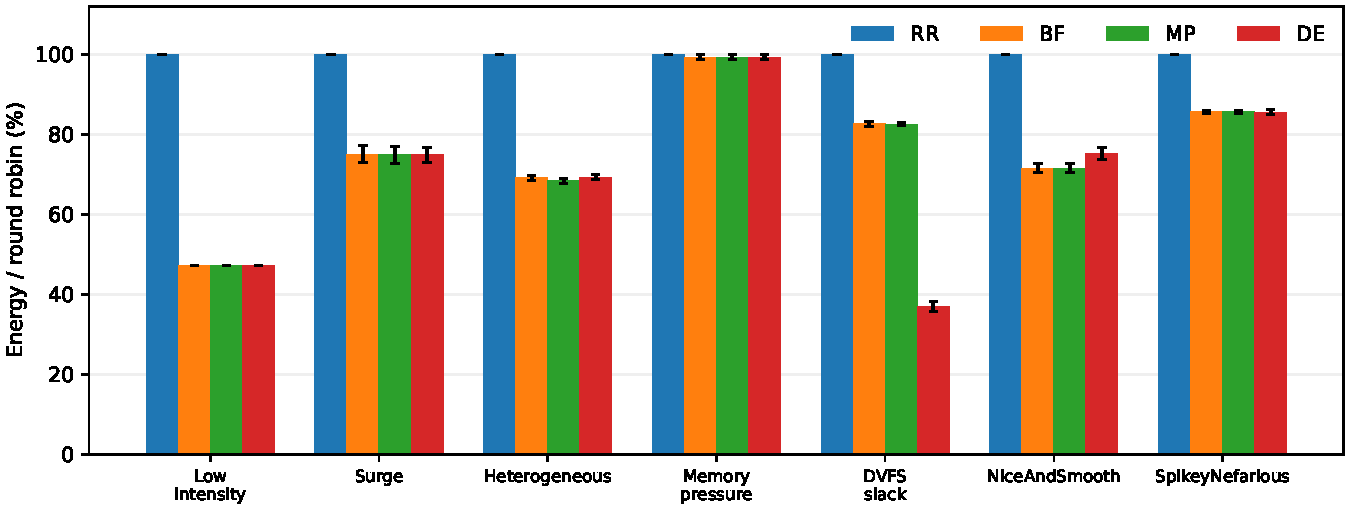
\includegraphics[width=\linewidth]{results/energy_comparison.pdf}
\small Figure 1. Energy relative to RR for paired seeds. Bars show the mean ratio;
error bars show its sample standard deviation across three seeds.
\end{center}

\newpage
\section*{Main study: measured energy and performance}
Policy abbreviations are \policies. Table 1 reports mean energy in \textbf{Wh}
($1\ \mathrm{Wh}=0.001\ \mathrm{kWh}$), giving readable values for these short
scenarios. These are simulator measurements, not estimates from DE's cost model.

\begin{center}
\small
\begin{tabular}{lrrrr}
\toprule
Workload & RR & BF & MP & DE \\
\midrule
Low intensity & 3.349 & 1.582 & 1.582 & 1.582 \\
Surge & 5.989 & 4.491 & 4.487 & 4.484 \\
Heterogeneous & 5.319 & 3.677 & 3.634 & 3.686 \\
Memory pressure & 0.806 & 0.800 & 0.800 & 0.800 \\
DVFS slack & 2.252 & 1.861 & 1.859 & 0.832 \\
NiceAndSmooth & 11.923 & 8.534 & 8.534 & 8.965 \\
SpikeyNefarious & 11.350 & 9.723 & 9.714 & 9.710 \\
\bottomrule
\end{tabular}

\\[4pt]Table 1. Mean cluster energy over three seeds (Wh).
\end{center}

\textbf{SLA and task completion.} All 84 main-study executions report zero misses
for every populated SLA class and zero memory warnings. The scheduler's shutdown
check confirms that its completed count equals \texttt{GetNumTasks()} and that
there are no pending or reserved jobs. Within each seed, completion counts agree
across policies. Main-study DE populations are 8--20 (low intensity), 313--379
(surge), 445--479 (heterogeneous), 76--81 (memory), 147--161 (DVFS), 69--90 (smooth),
and 712--772 (spiky). No admission failures were excluded from this study.

\begin{center}
\scriptsize
\setlength{\tabcolsep}{3pt}
\resizebox{\linewidth}{!}{\begin{tabular}{lrrrr}
\toprule
Workload & RR & BF & MP & DE \\
\midrule
Low intensity & 0.104/13.42/0.003 & 0.104/13.42/0.004 & 0.104/13.42/0.004 & 0.104/13.42/0.004 \\
Surge & 0.730/12.56/0.016 & 0.909/12.56/0.017 & 0.908/12.56/0.016 & 0.909/12.56/0.028 \\
Heterogeneous & 0.225/12.64/0.013 & 0.246/12.68/0.014 & 0.255/12.68/0.014 & 0.247/12.72/0.027 \\
Memory pressure & 0.810/7.34/0.004 & 0.940/7.50/0.005 & 0.940/7.50/0.004 & 0.940/7.50/0.007 \\
DVFS slack & 0.397/15.64/0.008 & 0.403/15.64/0.008 & 0.403/15.64/0.007 & 0.669/15.82/0.015 \\
NiceAndSmooth & 0.435/16.08/0.007 & 0.332/15.82/0.012 & 0.332/15.82/0.012 & 0.736/16.40/0.020 \\
SpikeyNefarious & 0.653/15.82/0.030 & 0.758/15.82/0.032 & 0.757/15.82/0.032 & 0.756/15.82/0.068 \\
\bottomrule
\end{tabular}
}
\\[4pt]\small Table 2. Each cell is mean response / simulated makespan / measured wall time,
all in seconds, averaged over the same three seeds. Wall times are environment dependent.
\end{center}

The low-intensity workload saves \textbf{52.75\%} with DE versus RR. BF and MP
match DE here: static power and idle capacity dominate, so DVFS adds no benefit.
In the surge workload DE saves \textbf{25.13\%} while all policies maintain the
observed SLA. Wake-up reservations ensure that bursts do not oversubscribe memory
or add work to a machine before its transition completes.

Heterogeneous work saves \textbf{30.70\%} with DE versus RR, but MP consumes less
energy than DE. The extra model detail does not establish dominance: DE estimates
CPU service conservatively and uses a heuristic GPU preference, while MP directly
favors small incremental power. Its source-based rule is competitive on this input.

The memory-limited scenario saves only \textbf{0.77\%} with DE. All three machines
remain needed for much of the run; unused cores do not imply enough memory to
consolidate. The result highlights why VM overhead and reservations are hard
constraints rather than soft penalties.

The DVFS scenario saves \textbf{63.06\%} with DE versus RR, and roughly 55\%
relative to the two P0 consolidation policies. Here reducing voltage/frequency
saves enough dynamic power to justify longer service times. Including static
power in the model avoids assuming that the slowest available state always wins.

On NiceAndSmooth, DE saves \textbf{24.81\%} over RR but uses about 5.0\% more energy
than BF/MP. A local placement estimate can favor a slower host and extend the
cluster's powered tail. SpikeyNefarious shows smaller, \textbf{14.45\%} DE savings;
under high occupancy, much of the installed capacity must remain active.

\newpage
\small
\section*{Longer runs, overload, and comparative conclusions}
The additional study uses the supplied seeds unchanged, once per policy and input.
Table 3 uses \textbf{kWh}, unlike Table 1. Big Small/BigSmall-1, Day/Day-1, and
SpikeyNefarious/SpikeyNefarious-1 are byte-identical pairs; only one of each pair
needs a separate measurement. TallShort, the hour scenarios, and Day additionally
test prolonged queues and scheduler scaling.

\begin{center}
\small
\begin{tabular}{lrrrr}
\toprule
Workload & RR & BF & MP & DE \\
\midrule
BigSmall & 0.02921 & 0.02773 & 0.02754 & 0.02773 \\
SpikeyMean & 0.02490 & 0.02425 & 0.02425 & 0.02425 \\
TallShort & 0.03524 & 0.03403 & 0.03419 & 0.03425 \\
GentlerHour & 7.26971 & 4.71368 & 4.71860 & 4.71449 \\
AnHour & 7.35318 & 4.83940 & 4.83958 & 4.74594 \\
Day & 64.10094 & 46.57883 & 46.58331 & 47.26487 \\
\bottomrule
\end{tabular}

\\[3pt]Table 3. Cluster energy on the additional supplied workloads (kWh).
\end{center}
\begin{center}
\small
\begin{tabular}{lrrrr}
\toprule
Workload & RR & BF & MP & DE \\
\midrule
BigSmall & 29.82/0.81 & 30.06/0.73 & 29.70/0.73 & 30.06/0.89 \\
SpikeyMean & 27.84/0.69 & 28.08/0.66 & 28.08/0.66 & 28.08/0.80 \\
TallShort & 34.68/1.03 & 34.74/0.91 & 35.04/0.91 & 35.04/1.04 \\
GentlerHour & 3603.48/2.23 & 3603.48/5.30 & 3603.48/5.34 & 3603.48/11.78 \\
AnHour & 3603.48/5.57 & 3603.48/9.94 & 3603.48/10.16 & 3603.48/48.70 \\
Day & 86400.72/28.63 & 86400.72/44.22 & 86400.72/53.42 & 86401.14/86.89 \\
\bottomrule
\end{tabular}

\\[3pt]Table 4. Simulated makespan / wall time (seconds), supplied seed.
\end{center}

\textbf{The overload limitation is observable.} All additional runs have zero
memory warnings and complete every generated task. The populated SLA classes
report zero misses except on TallShort. Its two bursts have a 1 ms mean interarrival
time and 3 s nominal runtime, producing 4,006 SLA0 tasks plus 82 SLA1 tasks on 160
cores of unequal speed. All four policies exceed the 5\% SLA0 miss allowance:
\begin{center}
\small
\begin{tabular}{lrr}
\toprule
Policy & SLA0 misses (\%) & SLA1 misses (\%) \\
\midrule
RR & 32.65 & 3.66 \\
BF & 34.17 & 3.66 \\
MP & 34.17 & 3.66 \\
DE & 34.10 & 3.66 \\
\bottomrule
\end{tabular}

\end{center}
This experiment is a failure to satisfy SLA0, not a successful compliant run.
EDF and P0 keep the system progressing but do not guarantee feasibility under
large backlogs. Reducing energy while ignoring these misses would give a misleading
ranking. The report makes no claim that a globally optimal schedule cannot do better.

\textbf{Validation and limits.} \texttt{make test} covers strict mock-interface
checks for small/heterogeneous clusters, multiple VM images, exact memory bounds,
asynchronous and immediate callbacks, EDF, best-effort aging, and all-task DVFS
bounds. It also performs 32 normal real-simulator runs, a repeatability comparison,
invalid-input checks, and a deliberately undersized configuration that must report
SLA misses. The implementation avoids deep sleep and migration; S1 wake latency
is a deliberate cost for lower risk. The timing margins and GPU preference are
heuristics. Workload-specific energy gains should not be generalized to arbitrary
hardware, tighter deadlines, or untested arrivals.

\small
\textbf{Reference [1].} A. Beloglazov, J. Abawajy, and R. Buyya,
\emph{Energy-aware resource allocation heuristics for efficient management of data
centers for Cloud computing}, Future Generation Computer Systems 28(5), 755--768,
2012, Algorithm 1, DOI: 10.1016/j.future.2011.04.017.
\href{https://clouds.cis.unimelb.edu.au/papers/Energy-Aware-CloudResourceAllocation-FGCS2012.pdf}{Author-hosted paper}.

\textbf{Attribution.} OpenAI Codex assisted with the scheduler implementation,
workload generation, tests, experiment scripts, analysis, and report text. The
supplied starter interfaces and simulator objects are course materials. MP's
conceptual source is [1]; no source code was copied from that paper. Measurements
come from the actual executable and retained logs, rather than generated examples.
\textbf{Comparative study.} RR offers a simple performance baseline but pays for
idle capacity. BF captures most static-power savings at low implementation cost.
MP's incremental-power rule is particularly competitive with heterogeneous machines.
DE provides the largest savings when core power and deadline slack justify DVFS,
while incurring more scheduler wall time and sometimes losing to simpler policies.
It is a useful default across the tested scenarios, with selectable alternatives
for evaluating these tradeoffs. No policy dominates all workloads; SLA feasibility
must remain part of any energy comparison.

\end{document}
